\documentclass[10pt, aspectratio=169]{beamer}

\setbeamertemplate{frametitle}[default][center]
\setbeamertemplate{navigation symbols}{}
\setbeamertemplate{footline}[frame number]
\setbeamertemplate{itemize items}[circle]

\setbeamercolor{block body alerted}{bg=alerted text.fg!10}
\setbeamercolor{block title alerted}{bg=alerted text.fg!20}
\setbeamercolor{block body}{bg=structure!10}
\setbeamercolor{block title}{bg=structure!20}
\setbeamercolor{block body example}{bg=green!10}
\setbeamercolor{block title example}{bg=green!20}
\setbeamertemplate{blocks}[rounded]%[shadow]

\makeatletter
\def\blfootnote{\xdef\@thefnmark{}\@footnotetext}
\makeatother

\title{Journal Club}
\author{Valentin Marteau}
\date{31.05.2022}

\begin{document}

\frame{\titlepage}

\begin{frame}{Paper}
\centering
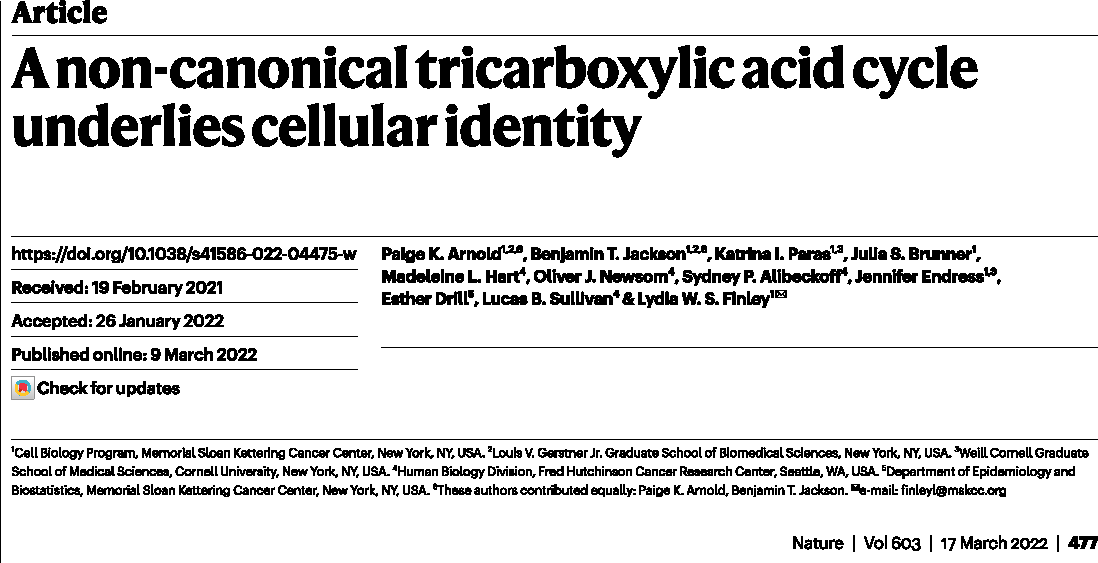
\includegraphics[width=0.9\textwidth]{figures/Arnold_2022_title.pdf}
\end{frame}

\begin{frame}{Aim}
\begin{columns}
\column{0.7\linewidth}

\begin{block}{\centering Tricarboxylic acid (TCA) cycle:}
\vspace{0.2cm}
    \begin{itemize}
        \item Central hub of cellular metabolism \\[0.1cm]
        \item Oxidation of nutrients for energy and metabolite production \\[0.1cm]
        \item Mammalian cells display diversity in TCA-cycle activity \\[0.1cm]
    \end{itemize}
\vspace{0.2cm}
\end{block}


\vspace{0.6cm}

\begin{itemize}
    \item[$\rightarrow$] \textbf{How is this diversity achieved?} \\[0.3cm]
    \item[$\rightarrow$] \textbf{Is the TCA cycle critical for establishing cell fate?}
\end{itemize}

\column{0.3\linewidth}
\centering
\includegraphics[width=0.9\textwidth]{figures/Martínez-Reyes_2020_fig2.pdf}\\[0.1cm]
\tiny{Martínez-Reyes \& Chandel; \textit{Nat. Commun.} (2020)}
\end{columns}
\end{frame}

\begin{frame}{DepMap project}

\blfootnote{
\includegraphics[width=0.15\textwidth]{figures/depmap_consortium_logo2.pdf}}
\end{frame}

\begin{frame}{Metabolic gene essentiality correlations across cancer cell lines}
\centering
\includegraphics[width=0.74\textwidth]{figures/Arnold_2022_figS1.png}
\end{frame}

\begin{frame}{Two modes of TCA-cycle metabolism}
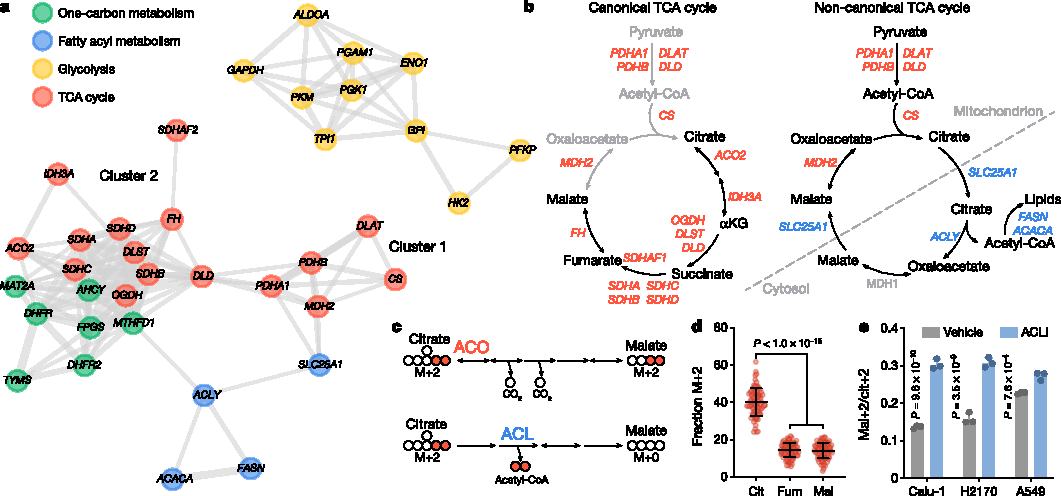
\includegraphics[width=\textwidth]{figures/Arnold_2022_fig1.pdf}
\end{frame}

\begin{frame}{ES cells engage a non-canonical TCA cycle}
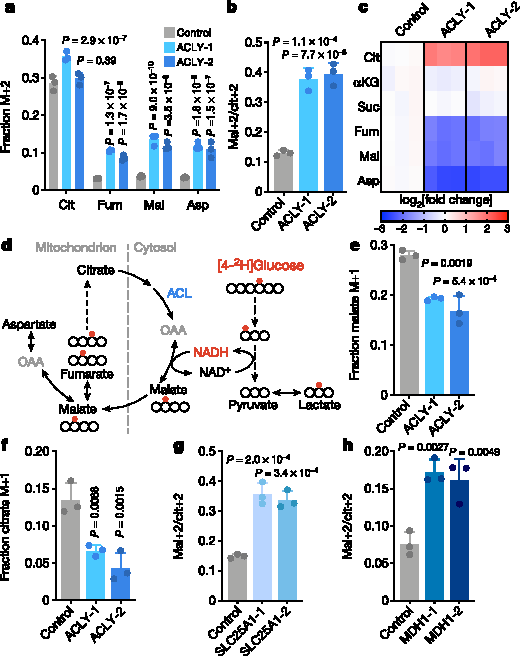
\includegraphics[width=0.4\textwidth]{figures/Arnold_2022_fig2.pdf}
\end{frame}

\begin{frame}{TCA-cycle choice is cell-state dependent}
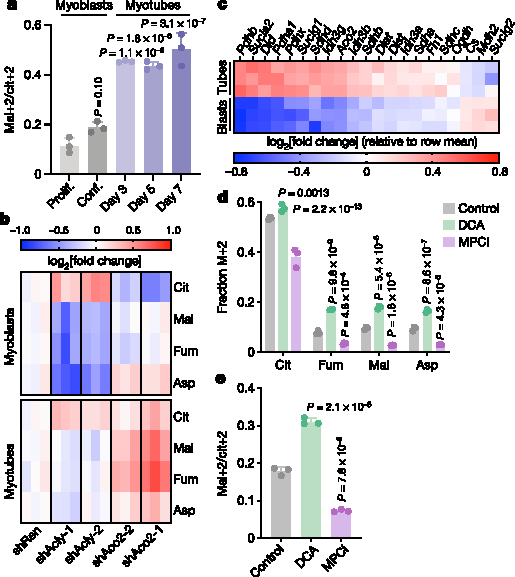
\includegraphics[width=0.4\textwidth]{figures/Arnold_2022_fig3.pdf}
\end{frame}

\begin{frame}{TCA-cycle switch after pluripotency exit}
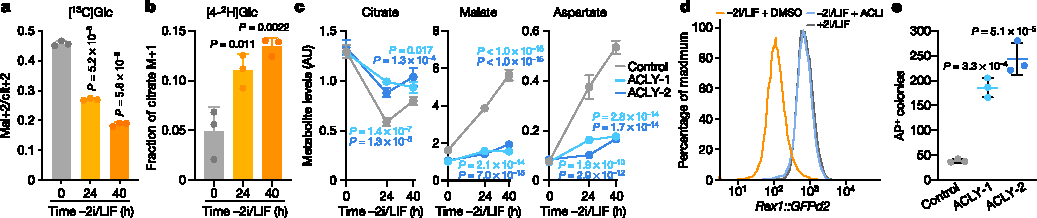
\includegraphics[width=\textwidth]{figures/Arnold_2022_fig4.pdf}
\end{frame}

\begin{frame}{Exit from pluripotency requires ACL}

\end{frame}

\begin{frame}{Summary}
\begin{itemize}
    \item[$\rightarrow$] \textbf{Identification of a non-canonical TCA cycle required for changes in cell state} \\[0.3cm]
    \item[$\rightarrow$] \textbf{Genetic co-essentiality mapping revealed gene cluster sufficient to compose alternative to canonical TCA-cycle}
    \item[$\rightarrow$] \textbf{}
\end{itemize}
\end{frame}

\begin{frame}{Questions to be addressed}

\end{frame}

\begin{frame}{Take home messages}

Include Otto Warburg Grant Proposal?
\end{frame}

\end{document}





